

\section{手拉手模型——旋转全等}
\subsection{手拉手模型的定义及基本结论}
\begin{custom}[explorecolor]{手拉手全等模型}
	所谓手拉手模型,是指\textcolor{red}{顶角相等},且有\textcolor{red}{公共顶点}的两个\textcolor{red}{等腰三角形}组成的图形,从中可以得到一个经典的全等模型:因为顶点相连的四条边,形象的可以看作两双手,所以通常称为“手拉手模型”.常见的有等边三角形共顶点,等腰直角三角形共顶点,正方形共顶点等几种,如下图所示。
	
	\begin{minipage}{0.3\textwidth}
		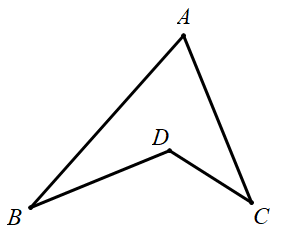
\includegraphics[scale=0.3]{figure/feibiao01.PNG}
	\end{minipage}
	\begin{minipage}{0.6\textwidth}
		结论\ding{192}:\textcolor{red}{$\angle BDC=\angle A+\angle B+\angle C$}\\
		结论\ding{193}:\textcolor{red}{$AB+AC>BD+CD$}
	\end{minipage}
\end{custom}

\subsection{手拉手模型的类型}
\subsection{一般等腰三角形手拉手}
\begin{minipage}{0.4\textwidth}
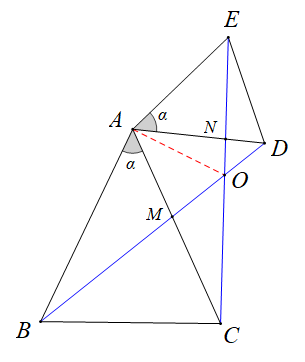
\includegraphics[scale=0.6]{figure/shoulashou01}
\end{minipage}
\begin{minipage}{0.6\textwidth}
  结论\ding{192}:\textcolor{red}{$\triangle ABD\cong \triangle ACE$};\\
  结论\ding{193}:\textcolor{red}{$BD=CE$};\\
  结论\ding{194}:\textcolor{red}{$\angle BOC=\angle BAC=\alpha$};\\
  结论\ding{195}:\textcolor{red}{$OA$平分$\angle BOE$};\\
  结论\ding{196}:\textcolor{red}{$\triangle ABM\sim \triangle OCM,\triangle AEM\sim \triangle ODN$};\\
   结论\ding{197}:\textcolor{red}{点$A,B,C,O$四点共圆,点$A,E,D,O$四点共圆}.
\end{minipage}
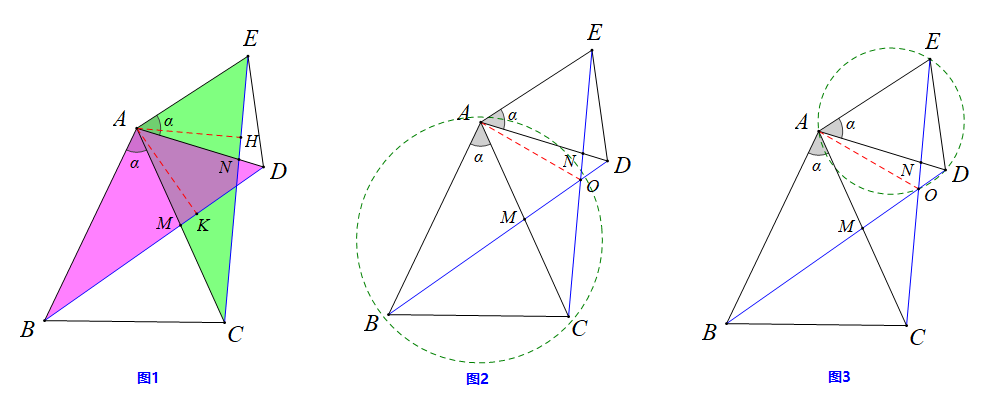
\includegraphics[scale=0.6]{figure/shoulashou02}
\subsection{等边三角形手拉手}
如图,直线$AB$的同侧作$\triangle ABD$和$\triangle BCE$都为等边三角形,连接$AE,CD$,二者交点为$H$,则有以下结论成立:

\begin{minipage}{0.4\textwidth}
	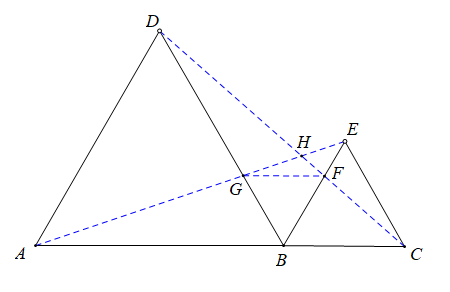
\includegraphics[scale=0.6]{figure/shoulashou03}
\end{minipage}
\begin{minipage}{0.6\textwidth}
 结论\ding{192}:\textcolor{red}{$\triangle ABE\cong \triangle DBC$};\\
结论\ding{193}:\textcolor{red}{$AE=DC$};\\
结论\ding{194}:\textcolor{red}{$\angle DHA=60^\circ$};\\
结论\ding{195}:\textcolor{red}{$\triangle AGB\cong \triangle DFB;\triangle EGB\cong \triangle CFB$};\\
结论\ding{196}:\textcolor{red}{连接$GF,\triangle BGF$是等边三角形};\\
结论\ding{197}:\textcolor{red}{$GF//AC$};\\
结论\ding{198}:\textcolor{red}{连接$HB$,$HB$平分$\angle AHC$};\\
结论\ding{199}:\textcolor{red}{$HC=HB+HE;HA=HC+HD$};\\
结论\ding{200}:\textcolor{red}{$\triangle DHG\sim \triangle ABG;\triangle EHF\sim \triangle CBF$};\\
结论\ding{201}:\textcolor{red}{点$A,B,H,D$四点共圆,点$C,B,H,E$四点共圆}.
\end{minipage}
\subsection{正方形手拉手}
\begin{minipage}{0.6\textwidth}
如图,四边形$ABCD$和四边形$CEFG$均为正方形,连接$BE,DG$,则有以下结论:

结论\ding{192}:\textcolor{red}{$\triangle BCE\cong \triangle DCG$};\\
结论\ding{193}:\textcolor{red}{$BE=DG,BE\perp DG$}.
\end{minipage}
\begin{minipage}{0.4\textwidth}
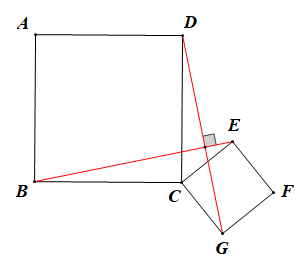
\includegraphics[scale=0.7]{figure/shoulashou04}
\end{minipage}

\subsection{习题演练}


